\documentclass[../main.tex]{subfiles}

\begin{document}

\subsection{Lenguaje de signos}

La aplicación será capaz de interpretar la lengua de signos americana (ASL). Dentro de esta lengua, se encargará de poder interpretar el alfabeto de letras. 

Dentro del alfabeto, se excluyen dos letras: la 'Z' y la 'J'. Debido a que su representación se realiza con un gesto, y no puede realizarse de forma estática. Por lo tanto, como se puede ver en la Figura \ref{figure1}, estas son las diferentes letras que podrá interpretar la aplicación.


\begin{figure}[h]
\centering 
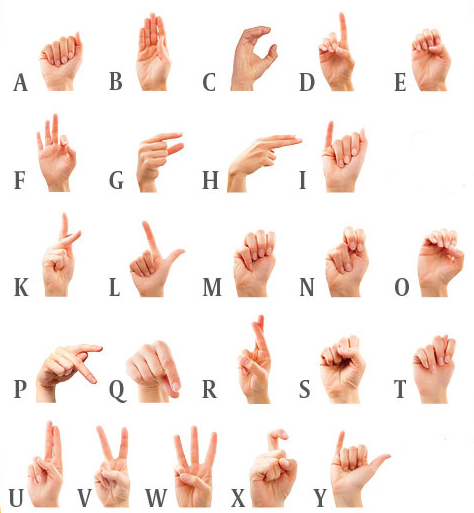
\includegraphics[width=0.7\textwidth]{images/alphabet_modify.png}
\caption{Imágenes de las 24 letras con su gesto en ASL \small Recuperado de: \url{https://deafchildren.org/2019/06/free-asl-alphabet-chart/}}
\label{figure1}
\end{figure}

\subsection{Extracción de características}

Para la generación de un modelo que sea capaz de interpretar signos, la parte más importante es la extracción de características.  Normalmente la extracción de características se realiza como paso previo al entrenamiento del modelo, y es realizado por el mismo componente que se encarga de compilar y entrenar el modelo. Pero en este proyecto se va a realizar en otro componente del sistema.

Las características que se van a utilizar para entrenar el modelo están basadas en las posiciones relativas de los dedos. Para ello, tendremos que detectar en una imágen donde está cada uno de los dedos, de forma que podamos obtener coordenadas para diferentes posiciones de los dedos y en base a estas coordenadas entrenar un modelo.

Este proceso de reconocimiento de imágenes con tanta precisión es un problema bastante complejo de resolver, pero dado que este proyecto es una aplicación para dispositivos iOS, se va a utilizar Apple Vision Framework para resolver este problema.

\newpage 

Apple Vision Framework: The Vision framework performs face and face landmark detection, text detection, barcode recognition, image registration, and general feature tracking. Vision also allows the use of custom Core ML models for tasks like classification or object detection~\cite{Vision}

Con el uso de Vision Framework, podremos detectar si existe una mano en una imagen, y a su vez detectar las posiciones relativas de cada uno de los dedos. Utilizamos estos datos como entrada para el entrenamiento de un modelo de Deep Learning realizado en Keras.


\subsection {Modelo Deep Learning}

Se construye un modelo de Deep Learning que utiliza como entrada los datos generados por Vision Framework para entrenar el modelo. Se utiliza Python y Keras como herramientas. El modelo es una red neuronal con diferentes capas que tiene como entrada 42 valores, representando diferentes coordenadas de los dedos de una mano, y tendrá como salida una distribución de probabilidad que indica la probabilidad de que la entrada pertenezca a cada una de las 24 letras que estamos intentando identificar. 

Se realiza un proceso de entrenamiento y mejora del modelo, mediante Fine-Tuning de hiper-parámetros, y como último paso tendremos que convertir el modelo generado a un formato compatible con dispositivos iOS: Core ML, para ello se utiliza la herramienta Core ML Tools~\cite{COREMLTOOLS}.

Core ML: Core ML is an Apple framework to integrate machine learning models into your app. Core ML provides a unified representation for all models. Your app uses Core ML APIs and user data to make predictions, and to fine-tune models, all on the user’s device. Core ML optimizes on-device performance by leveraging the CPU, GPU, and Neural Engine while minimizing its memory footprint and power consumption. Running a model strictly on the user’s device removes any need for a network connection, which helps keep the user’s data private and your app responsive~\cite{COREML}

\subsection { Dataset }

Se utilizan diferentes datasets para la extracción de características. A su vez, conforme avanza el entrenamiento y se obtienen los resultados en las diferentes predicciones de las letras, se revisan aquellas imágenes en las que el modelo está teniendo problemas para acertar en sus predicciones. Por lo tanto, el dataset final será una mezcla de los siguientes datasets tras un proceso de refinado para obtener los mejores resultados.

Se han utilizado los siguientes dataset:

\begin{enumerate}
    \item Image data set for alphabets in the American Sign Language~\cite{ASLALPHABET}.
    \item ASL Alphabet Images with a variety of backgrounds for validating a model~\cite{ASLALPHABET2}.
    \item Significant (ASL) Sign Language Alphabet Dataset~\cite{ASLALPHABET4}.
    \item ASL Sign Language Alphabet Pictures [Minus J, Z]~\cite{ASLALPHABET5}.
    \item American Sign Language Alphabet (Static)]~\cite{ASLALPHABET6}.
    \item Dataset propio con algunas imágenes
\end{enumerate}

\subsection { API REST }

Se utiliza un proyecto realizado con Python y Django que servirá para almacenar los diferentes datasets, así como proporcionar acceso vía web a la imágenes de cada uno. También proporcionará un API REST que permite obtener todos los enlaces a la imágenes organizados por letras. 

\subsection { Training App}

Para la extracción de características se utiliza Vision Framework, este framework está solamente disponible en dispositivos iOS, por lo que se realiza una aplicación iOS cuya utilidad es exclusivamente la extracción de características. 

Esta aplicación conectará con el API REST para obtener las imágenes a analizar, realizará una extracción de características de las imágenes, y proporcionará los resultados en formato .csv.
Este producto se realizará en una app diferente porque no debe formar parte del producto principal, que debe centrarse únicamente en interpretar ASL.

\subsection{ ASL Interpreter App }

Será el producto final y la aplicación que utilizará el usuario final. Utiliza el Modelo de Deep Learning generado por otro componente y su función es permitir diferentes entradas como puede ser usar de la cámara del dispositivo o seleccionar vídeos, y realizar predicciones. 
Las predicciones obtenidas por el modelo, pasarán por un proceso de comparar predicciones consecutivas para obtener resultados más fiables, y mostrará por pantalla los resultados obtenidos.

\end{document}